\documentclass{article}

% Load the unmodified official ICLR 2027 submission style from the local
% template package supplied with this repository.
\makeatletter
\def\input@path{{iclr2027/}}
\makeatother
\usepackage{iclr2027_conference,times}
\usepackage{amsmath,amssymb}
\usepackage{booktabs}
\usepackage{graphicx}
\usepackage{microtype}
\usepackage{xurl}
\usepackage{xcolor}
\usepackage[hidelinks]{hyperref}

\newcommand{\deltas}{\Delta S}
\newcommand{\model}{\textsc{Pythia}}

\title{Intervention-Conditioned Layer Fragility Across Language-Model Pretraining}
\author{Anonymous Authors}

% Anonymous submission: do not enable \iclrfinalcopy.

\begin{document}
\maketitle

\begin{abstract}
Interventions on neural-network components are often interpreted as measuring
properties such as redundancy or robustness, yet recent work shows that the
conclusion can depend on the intervention protocol. We test whether such
protocol dependence can be reduced to differences in output-level functional
damage. Our assay measures the fraction of intact next-token top-1 predictions
preserved after an interior-block intervention across independently pretrained
small \model{} models. The early-to-late block-bypass response replicates across
nine 160M runs, a held-out run, a 70M scale, and WikiText-2 and HellaSwag-derived
evaluation streams. Within residual attenuation, matched comparisons show that
KL/NLL predictive damage discriminates top-1 damage more strongly than raw
activation displacement. However, prospective joint KL/NLL matching does not
make block bypass and norm-controlled activation noise interchangeable: a
corrected family residual of $-0.0168$ remains across five runs. A frozen block
of simple output-logit and decision-boundary features accounts for only 20.2\%
of that residual. These results support a bounded methodological conclusion:
in the tested setting, intervention responses are conditioned on how a model is
perturbed and cannot be summarized by raw magnitude or matched predictive
damage alone. We do not identify a causal mechanism, establish downstream
capability loss, or claim generality beyond the tested small-model regime.
\end{abstract}

\section{Introduction}

Interventions---removing a layer, patching an activation, or injecting
noise---are widely used to infer redundancy, necessity, robustness, or causal
roles in neural networks. Such interpretations are strongest when reasonable
intervention procedures agree and weaker when the response depends on the
measurement protocol.

This concern is established empirically. Language models can preserve many
next-token predictions after layer deletion or swapping
\citep{lad2025remarkable}, while \citet{garcia2026nofreeswap} shows that
output-grounded layer equivalence changes across training and differs between
replacement and interchange. Intervention audits also show dependence on the
comparator and matching procedure \citep{luo2026steercheck}. We therefore ask
a narrower question: \emph{can protocol-dependent responses be explained by
differences in functional predictive damage?}

The explanation is plausible. Nominally equal interventions can change output
distributions differently, while interventions far apart in activation space
can be close in function space. If matching forward KL and target-token NLL
removes protocol dependence, intervention identity adds little beyond a
severity budget. If not, raw size and those output-level measures are
insufficient summaries.

We study independently pretrained 70M- and 160M-parameter \model{} models
\citep{biderman2023pythia}. For a fixed corpus and checkpoint, we intervene on
an interior block and measure the retained fraction $S$ of intact next-token
top-1 predictions; $D_S=1-S$ is top-1 damage and
$\deltas=S_{\mathrm{late}}-S_{\mathrm{early}}$ is the training endpoint change.
This operational metric is not new: it belongs to the relative-accuracy family
\citep{lad2025remarkable} and complements the divergent-token rate on identical
positions \citep{deiseroth2024dtm}.

The block-bypass endpoint is negative in all nine 160M runs, including a
prospectively held-out run, and repeats at 70M and on a HellaSwag-derived
stream. This establishes a stable outcome, not novelty for the broad training
phenomenon. Within residual attenuation, complementary matching shows that
KL/NLL damage is more informative than raw activation displacement, without
establishing KL/NLL causality.

The central test prospectively targets activation-noise strengths, using only
KL and NLL, to match block interventions by run, checkpoint, and layer. After a
tie-handling inconsistency was withdrawn and repaired, the canonical analysis
retains a family residual of $-0.0168$ (run-bootstrap 95\% interval
$[-0.0200,-0.0126]$): matched activation noise produces less top-1 damage than
block attenuation on average. A frozen output-logit and decision-boundary
feature block reduces this residual by 20.2\% but does not eliminate it.

Our contributions are exactly three:
\begin{enumerate}
    \item We establish an independently replicated empirical base for a fixed
    block-bypass response across two small \model{} scales and two English
    evaluation streams, including held-out, confidence, and layer controls.
    \item Complementary magnitude- and damage-matched contrasts show that
    output-level predictive damage is more informative than raw activation
    displacement within the frozen residual-attenuation assay.
    \item Prospective joint KL/NLL targeting and a corrected deterministic
    top-1 analysis show that predictive-damage matching does not eliminate the
    block/noise difference; simple output geometry explains only part of it.
\end{enumerate}

We do not infer universal specialization, large-model scaling, downstream
capability loss, KL/NLL causality, or an identified internal mechanism.

\section{Related Work}

\paragraph{Layer redundancy and protocol dependence.}
Layer deletion and swapping can preserve substantial next-token behavior
\citep{lad2025remarkable}; depth-pruning criteria likewise remove some
final-model layers with limited aggregate degradation \citep{men2025shortgpt}.
Our closest neighbor is \citet{garcia2026nofreeswap}, who shows that replacement
and interchange yield different output-grounded gaps across Pythia checkpoints.
That work occupies the broad protocol- and training-dependence claim. We ask
whether two intervention families become interchangeable after matching output
KL and NLL across independent pretraining runs.

\paragraph{Training-dependent perturbation fragility.}
Quantization degradation varies across pretraining and learning-rate phases
\citep{catalantatjer2026training}; activation-noise fragility can change after
probe accuracy saturates \citep{reblitzrichardson2026fragility}, and
layer-specific noise reveals heterogeneous learning dynamics
\citep{borras2022walking}. We therefore claim neither generic novelty for
training-dependent fragility nor a smooth training law.

\paragraph{Parameter, activation, and function space.}
Network composition, normalization, location, and direction decouple raw
perturbation size from functional change. Conversely, norm dominates recent
gradient-free language-model adaptation experiments in their specific regime
\citep{kim2026norm}. Our result rejects only a pure raw-displacement account
within the frozen attenuation assay. Forward KL, NLL change, and top-1 damage
share logits, so their alignment remains descriptive without controlled
contrasts.

\paragraph{Mechanistic and matched interventions.}
Activation patching and editing depend on corruption, metric, and intervention
design \citep{zhang2023patching,makelov2024subspace}; self-repair adds further
architecture- and prompt-specific dependence \citep{rushing2024selfrepair}.
SteerCheck is the closest methodological collision: it prospectively matches
off-target KL across steering comparators and retains direction/family
structure \citep{luo2026steercheck}. We do not claim matched-KL auditing as new;
we target joint KL/NLL for training-conditioned block substitutability and add
independent-run replication and explicit assay repair.

\paragraph{Prediction-disagreement metrics.}
The divergent-token metrics of \citet{deiseroth2024dtm} measure argmax changes
under pruning and quantization. On identical teacher-forced positions, our $S$
is one minus such a disagreement rate; novelty is claimed only for the
controlled result built around it.

\section{Experimental Setup}
\label{sec:setup}

\paragraph{Models, data, and statistical units.}
We study independent PolyPythias replicas from the \model{} suite
\citep{biderman2023pythia}: nine 160M runs form the principal trajectory, five
70M runs provide scale replication, and five or six 160M runs support the
controlled comparisons. The independent pretraining run is the scientific
replicate; tokens, layers, pairs, and evaluation selections are not treated as
independent. The primary WikiText-2 and cross-corpus HellaSwag-derived streams
are fixed teacher-forced sequences with the same tokenizer and 4,608 predicted
positions per checkpoint. Exact run/checkpoint allocations and selection
details are in Appendix~\ref{app:contract}.

\paragraph{Interventions.}
For block output $b(x)$ with residual input $x$, residual attenuation is
\begin{equation}
  \tilde b_\alpha(x)=b(x)-\alpha\,[b(x)-x],
\end{equation}
with $\alpha\in\{0.25,0.50,0.75,1.00\}$; $\alpha=1$ is block bypass. We
intervene on blocks 1--10 of the 12-block 160M architecture. The second family
adds a frozen random direction after the intact block with scale $\beta$
normalized by the local activation norm and averages directions within cell.

\paragraph{Agreement and training response.}
For intact distribution $p$ and intervened distribution $q_I$ on fixed
teacher-forced positions $t$, define
\begin{align}
 S(I,c) &= |T|^{-1}\sum_{t\in T}\mathbb{1}[\hat y_{c,t}=\hat y_{I,c,t}],\\
 D_S(I,c)&=1-S(I,c),\\
 \deltas(I)&=S(I,c_{\rm late})-S(I,c_{\rm early}),
\end{align}
where each $\hat y$ is the lowest-index token among exact maximum logits. The
core statistic averages over frozen interior layers and evaluation selections;
negative $\deltas$ means lower retained top-1 agreement late in training.

\paragraph{Damage and magnitude.}
We measure
\begin{align}
 D_{\rm KL}(I)&=\mathbb{E}_t\,\mathrm{KL}(p_t\Vert q_{I,t}),\\
 D_{\rm NLL}(I)&=\mathrm{NLL}(q_I)-\mathrm{NLL}(p).
\end{align}
Raw magnitude is the local relative residual-change norm; absolute activation
RMS is a sensitivity measure. These are descriptors, not assumed causes.

\paragraph{Matching and uncertainty.}
Within residual attenuation, magnitude matching constrains relative norm while
requiring functional-damage separation; damage matching calipers joint KL/NLL
while requiring location or magnitude separation. Pairing is deterministic,
within run/checkpoint, and without reuse. For the cross-family test, each block
cell defines a joint KL/NLL target. An outcome-blind deterministic search uses
only noise strength, KL, NLL, and technical diagnostics; strict `Class A'
requires both damage targets to meet their frozen relative calipers. The
primary residual is
\begin{equation}
 R_{\rm family}=\operatorname*{mean}_{r}
 \operatorname*{median}_{i\in r}[D_S^{\rm noise}(i)-D_S^{\rm block}(i)],
\end{equation}
with practical-equivalence band $\pm0.010742$. Exact calipers are reported in
Appendix~\ref{app:contract}. Intervals bootstrap independent-run summaries;
fixed intact-confidence bins, exclusions, and contrasts were frozen before
confirmatory outcomes.

\section{A Reproducible Intervention-Conditioned Response}
\label{sec:repro}

We first establish that the outcome used for mechanism discrimination is not a
single-checkpoint or single-run accident. This section is an empirical base for
the functional-damage question; it is not presented as discovery of the broad
training phenomenon.

\begin{table}[t]
\centering
\scriptsize
\caption{Selected validated results. Intervals bootstrap independent-run summaries.}
\begin{tabular}{@{}p{0.29\columnwidth}p{0.43\columnwidth}p{0.15\columnwidth}@{}}
\toprule
Result & Estimate & Replicates \\
\midrule
WikiText-2 $\deltas$ & $-0.1035$ [$-0.1115,-0.0958$] & 9/9 \\
HellaSwag $\deltas$ & $-0.0793$ [$-0.0885,-0.0677$] & 6/6 \\
Magnitude-matched contrast & $+0.0430$ [$0.0354,0.0525$] & 6/6 \\
Damage-matched contrast & $+0.0025$ [$-0.0009,0.0058$] & 4/6 \\
Corrected family residual & $-0.0168$ [$-0.0200,-0.0126$] & 5/5 \\
Geometry-adjusted residual & $-0.0134$ [$-0.0176,-0.0092$] & 5 runs \\
\bottomrule
\end{tabular}
\label{tab:key-results}
\end{table}


\paragraph{Independent runs and held-out prediction.}
Across nine independent 160M pretraining runs, every late-minus-early
block-bypass change is negative. Mean $\deltas$ is $-0.10353$, with a
run-bootstrap 95\% interval $[-0.11149,-0.09585]$; the median is $-0.10410$.
Run 9 was prospectively held out before its weights were evaluated. Its
$\deltas=-0.11895$ has the predicted sign and lies inside the frozen prediction
interval $[-0.13463,-0.06366]$. Intact NLL improves from an early-run mean of
3.878 to a late-run mean of 3.726, so the endpoint is not explained by a failure
to learn next-token prediction.

The direction is broad across the tested locations: all 90 run--interior-layer
endpoint changes are negative, and all ten layer medians are negative. The
magnitude is not uniform; layer medians range from $-0.0653$ to $-0.1838$.
Accordingly, we claim broad sign support, not location invariance.

\paragraph{Confidence control.}
Top-1 agreement is mechanically related to intact confidence. We therefore
repeat the endpoint comparison within five fixed intact-confidence bins. All
45 eligible run--bin changes are negative, with mean matched change $-0.11388$.
This control conditions on a coarse observable and does not fully match token
difficulty.

\paragraph{Scale and corpus boundaries.}
Five independent 70M runs reproduce the direction (5/5 negative; median
$\deltas=-0.14334$, 95\% interval $[-0.15385,-0.11030]$). This is replication at
two small scales inside one architecture family, not a scaling law.

On the HellaSwag-derived stream, all six 160M runs are negative, with mean
$\deltas=-0.07926$ and 95\% interval $[-0.08851,-0.06767]$. All 30 confidence-
bin changes are also negative. The absolute effect is 0.766 times the
WikiText-2 mean (95\% interval $[0.645,0.880]$): the direction repeats but the
magnitude is corpus-dependent. HellaSwag is easier and more confident under the
frozen stream, so the comparison does not imply corpus invariance.

\begin{figure*}[t]
\centering
\begin{minipage}[t]{0.32\textwidth}\centering
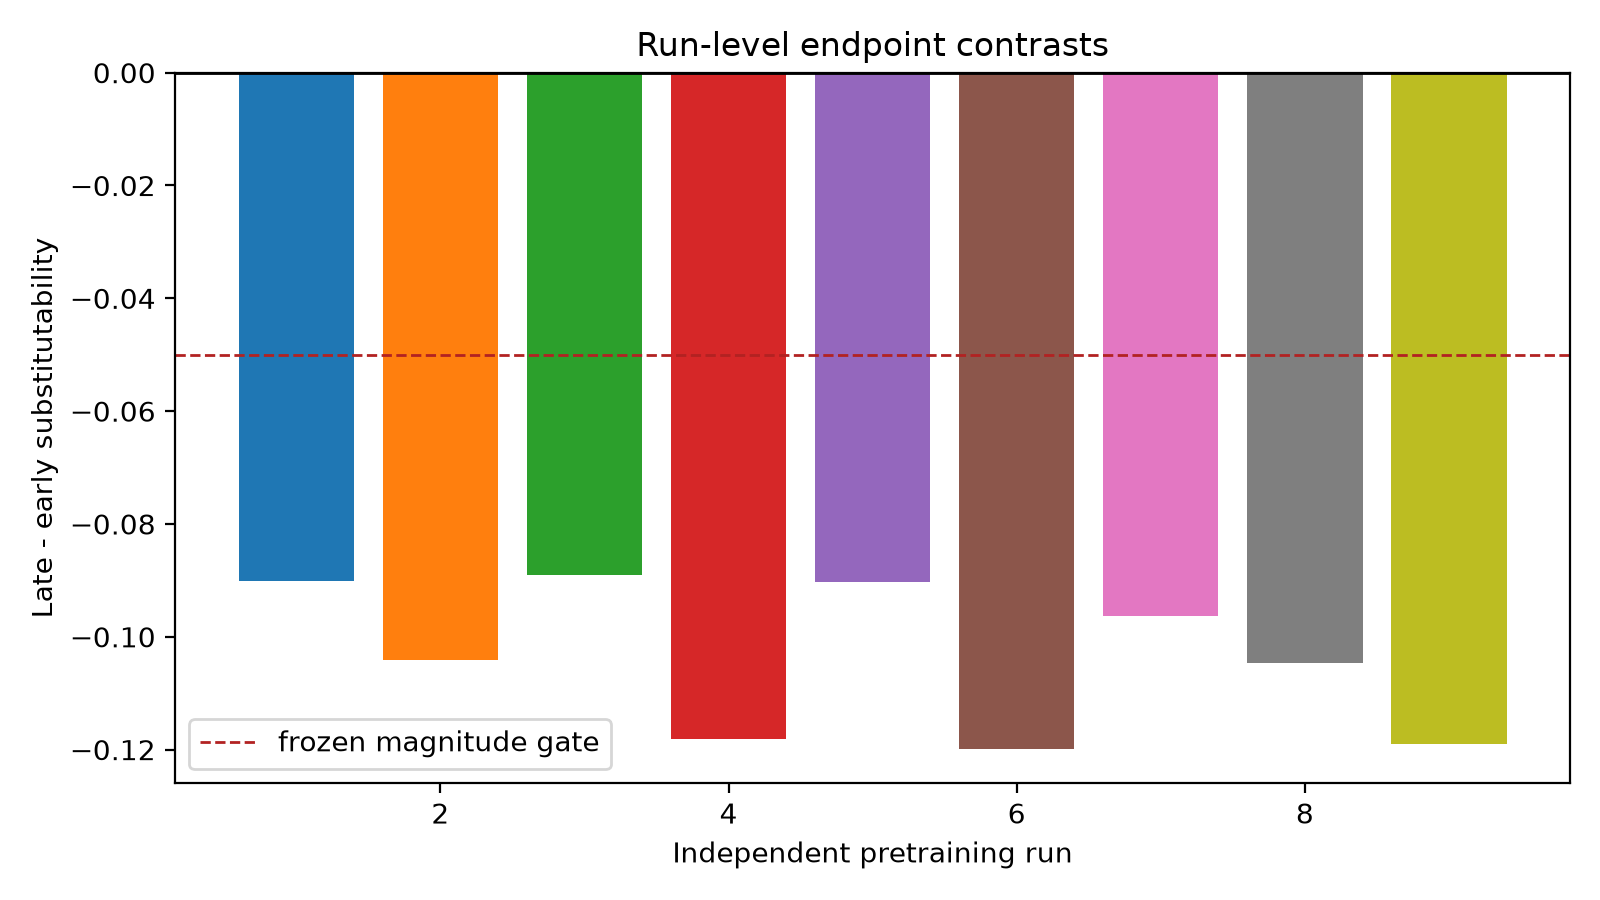
\includegraphics[width=\linewidth]{figures/draft2/fig1_pythia160.png}
\\[-2mm]\small (a) Nine independent 160M runs
\end{minipage}\hfill
\begin{minipage}[t]{0.32\textwidth}\centering
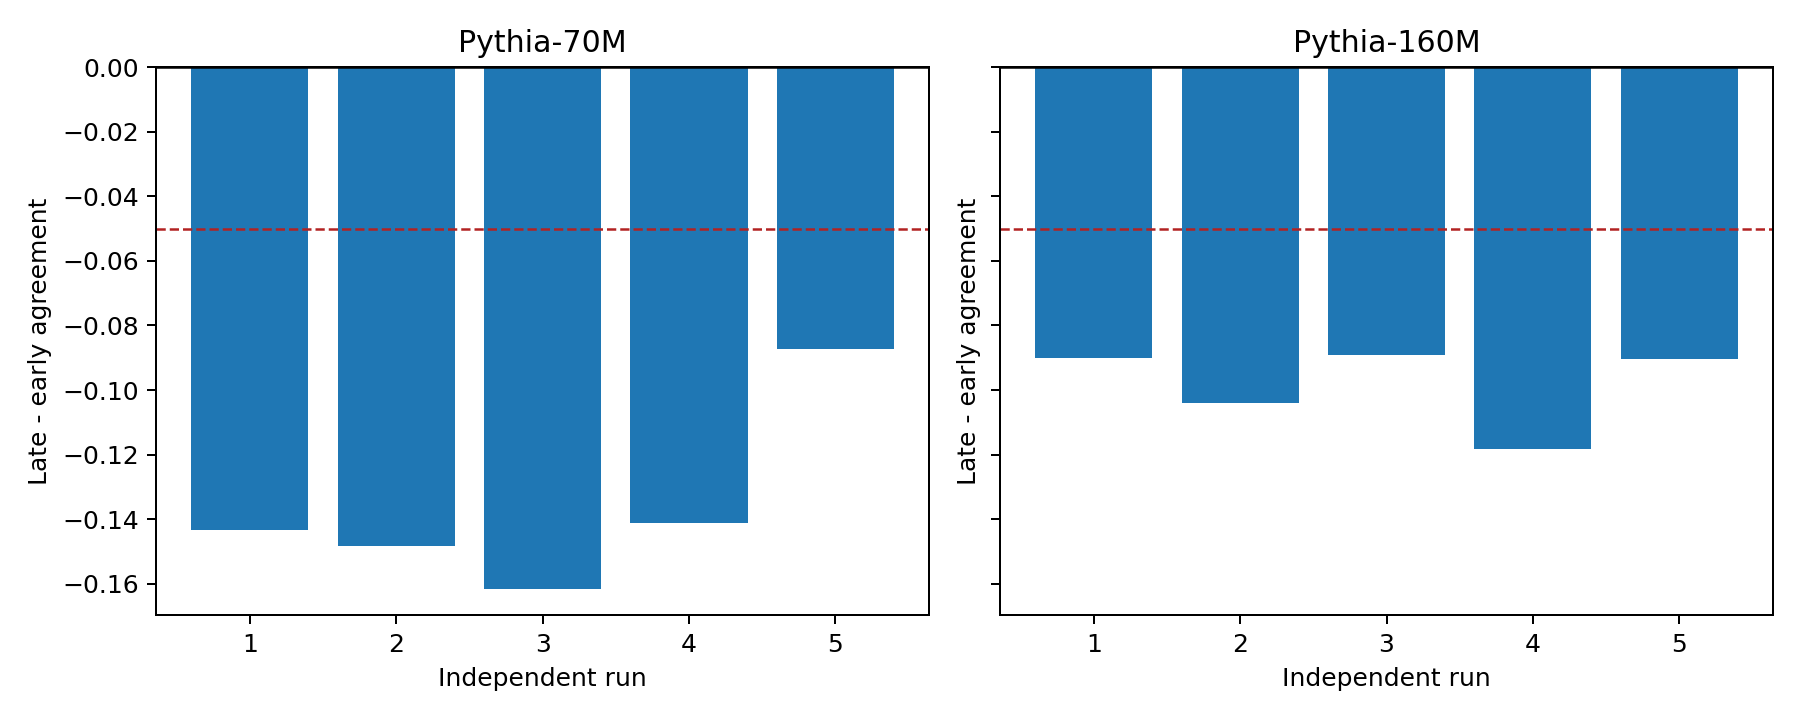
\includegraphics[width=\linewidth]{figures/draft2/fig1_pythia70.png}
\\[-2mm]\small (b) Five independent 70M runs
\end{minipage}\hfill
\begin{minipage}[t]{0.32\textwidth}\centering
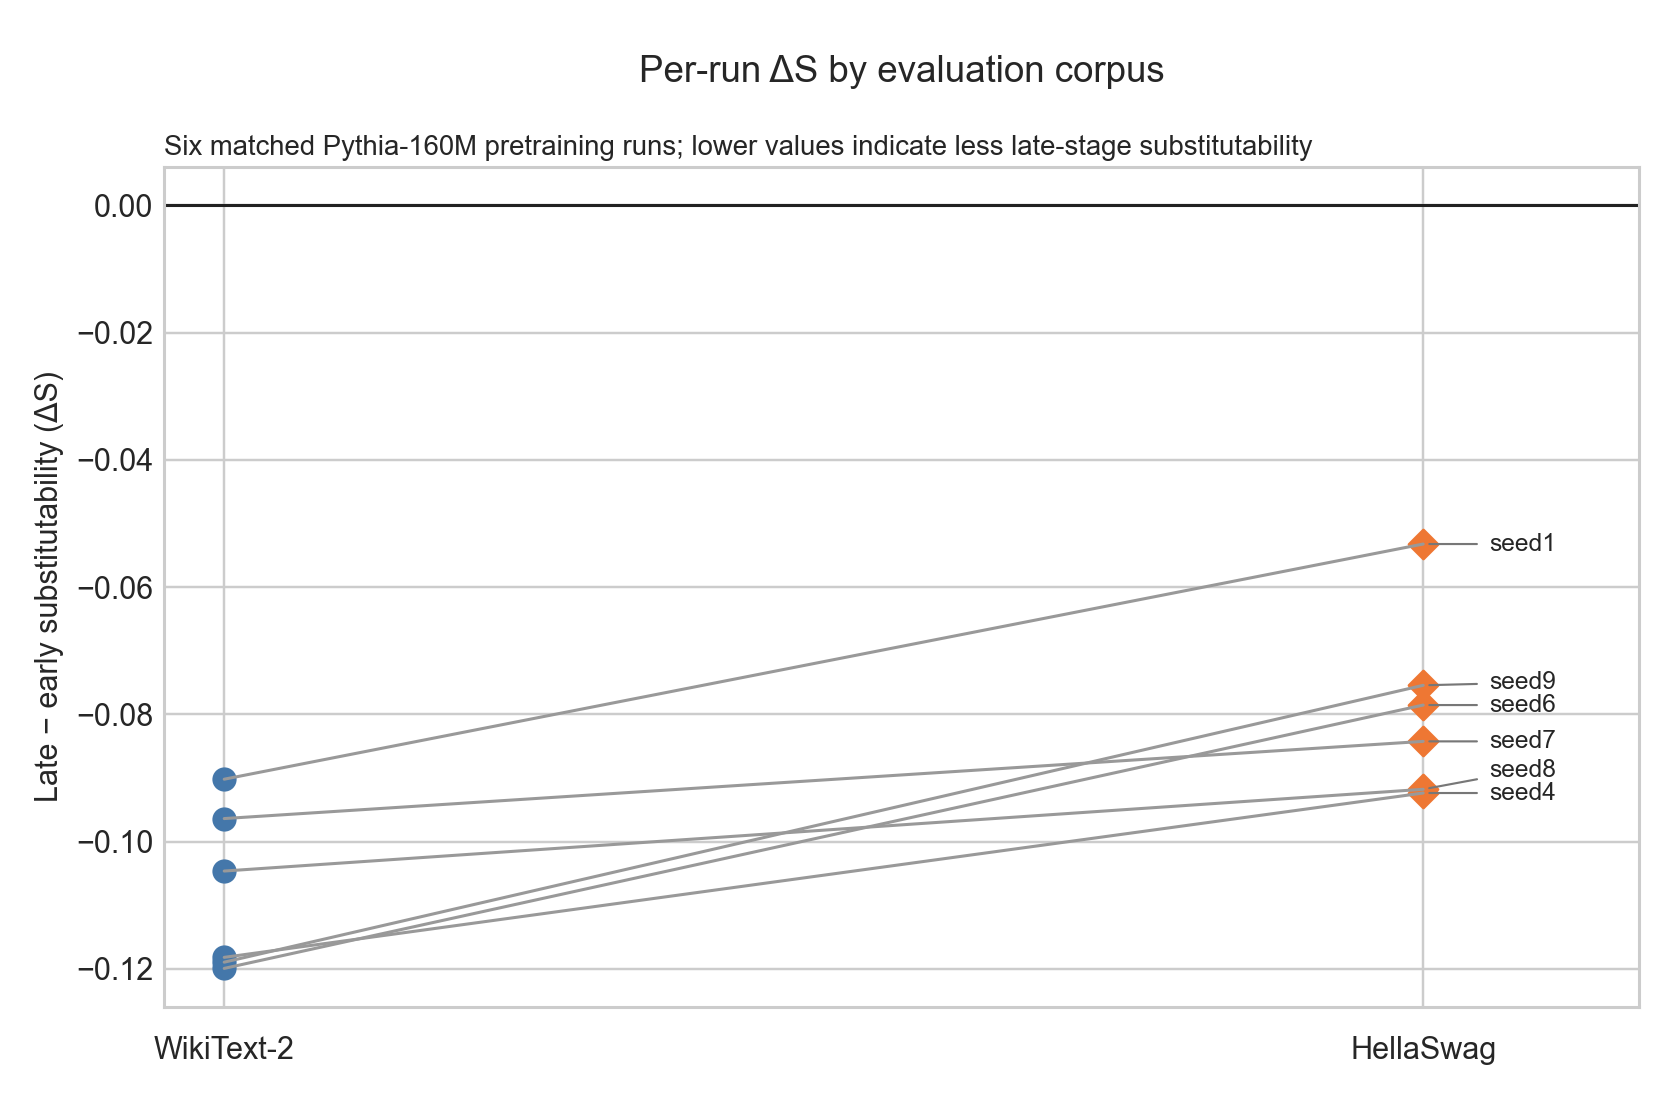
\includegraphics[width=\linewidth]{figures/draft2/fig1_hellaswag.png}
\\[-2mm]\small (c) HellaSwag-derived stream
\end{minipage}
\caption{\textbf{Empirical base.} The endpoint direction repeats across
independent runs, two small scales, and two evaluation streams. Panels reuse
sealed ARC figures without recomputing outcomes. Differences in magnitude are
not interpreted as invariance or a scaling law.}
\label{fig:repro}
\end{figure*}

Taken together, these checks justify using the endpoint response as a stable
outcome for the controlled comparisons that follow. They do not establish why
the response changes.

\section{Functional Damage Explains More Than Raw Magnitude}
\label{sec:damage}

We next discriminate between two simple descriptions of the response. A raw-
magnitude account predicts that interventions moving the local activation by a
similar amount should produce similar top-1 damage. A functional-damage account
instead predicts that the change in output distribution is the more informative
quantity. Because all variables are observational consequences of an
intervention, we use matched contrasts rather than interpreting raw
correlations.

\subsection{Magnitude-matched comparison}

The primary arm contains 185 disjoint pairs formed within run and checkpoint.
Their median relative-magnitude ratio is 1.019, while the median absolute KL and
NLL-damage separations are 0.087 and 0.098. In 94.6\% of pairs, the higher-KL
member also has higher NLL damage. The mean run-median difference in top-1
damage is $+0.04297$ (95\% interval $[0.03537,0.05246]$), positive in all six
runs and all three prospectively confirmatory runs. An absolute-RMS matching
sensitivity is stronger rather than weaker.

Thus, approximately equal local displacement does not equalize the response
when functional damage differs. The contrast holds within all five intact-
confidence bins, although fixed bins are not exact propensity matches.

\subsection{Damage-matched comparison}

The reverse arm contains 162 disjoint pairs with median absolute KL and NLL
gaps 0.0050 and 0.0070. Their median magnitude ratio is 1.129. The mean
run-median top-1 contrast is $+0.00246$, with a 95\% interval
$[-0.00090,0.00575]$. A stricter subset of 37 pairs with magnitude ratio at
least 1.25 has contrast $-0.00054$ and interval $[-0.00456,0.00371]$.
Checkpoint-level signs in this stricter subset are heterogeneous.

The two contrasts have a clear ordering: in this attenuation family,
functional-damage separation survives raw-magnitude matching, whereas
raw-magnitude separation leaves little stable contrast after joint KL/NLL
matching. This weakens a pure raw-displacement account. It does not show that
raw magnitude is generally irrelevant: the observational regression retains a
magnitude coefficient, location retains secondary structure, and the second
intervention family behaves differently.

\begin{figure*}[t]
\centering
\begin{minipage}[t]{0.48\textwidth}\centering
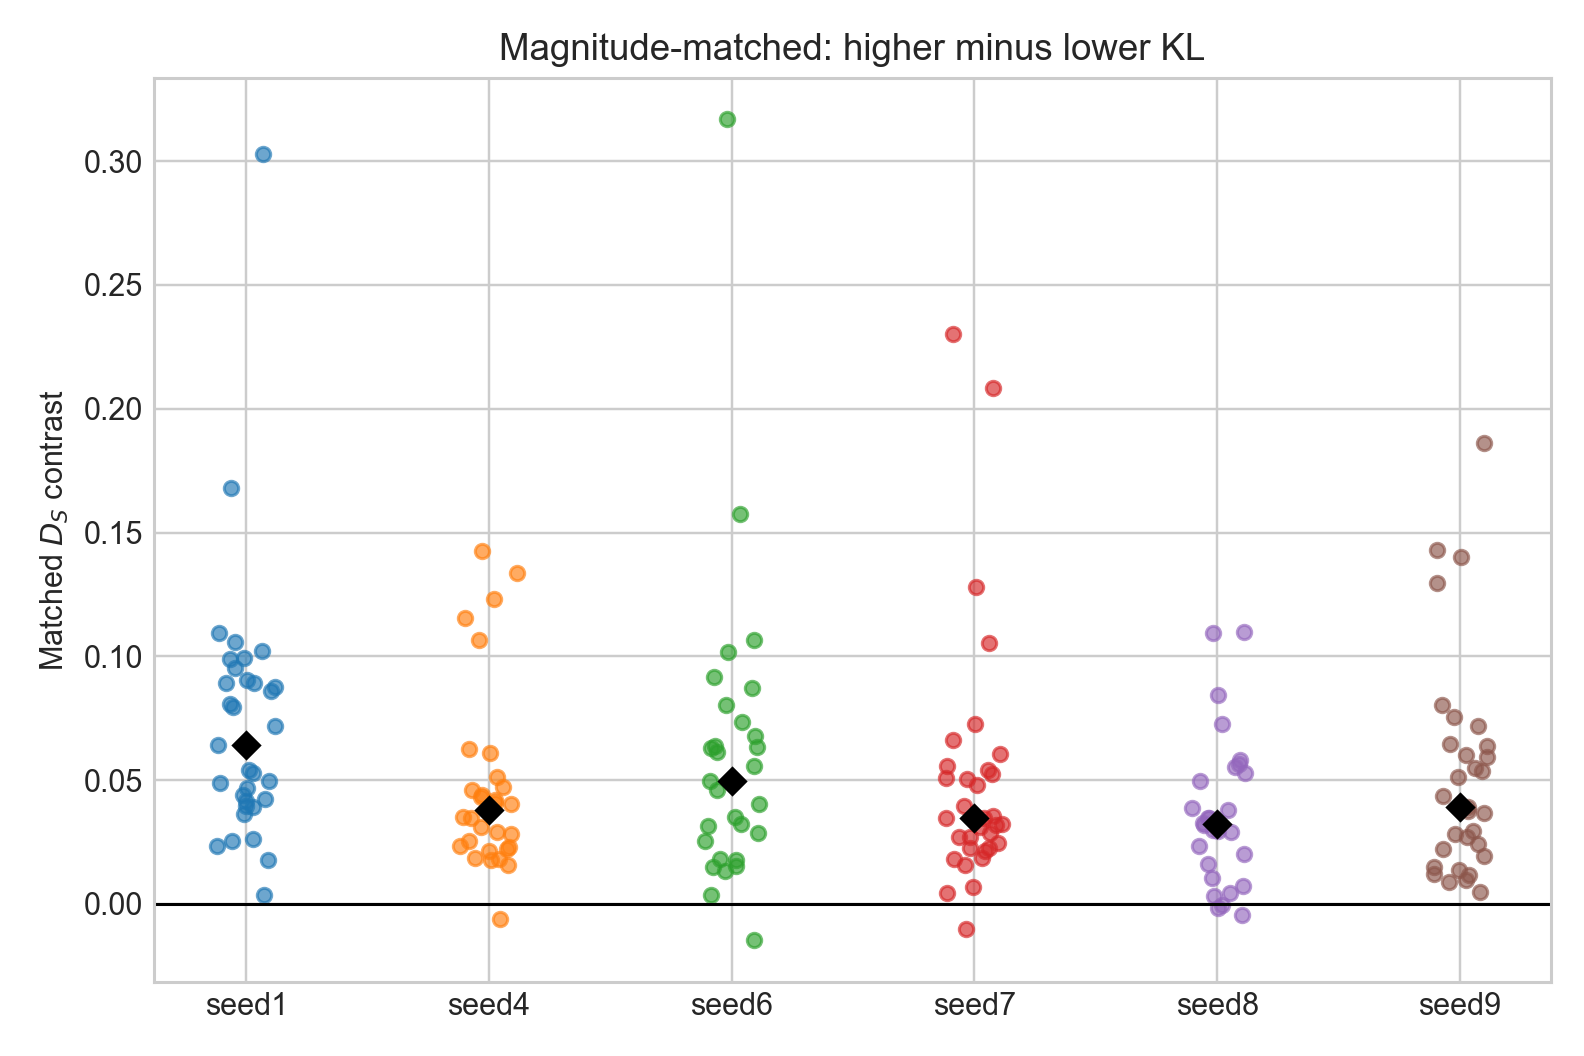
\includegraphics[width=\linewidth]{figures/draft2/fig2_magnitude_matched.png}
\\[-2mm]\small (a) Similar raw displacement, different functional damage
\end{minipage}\hfill
\begin{minipage}[t]{0.48\textwidth}\centering
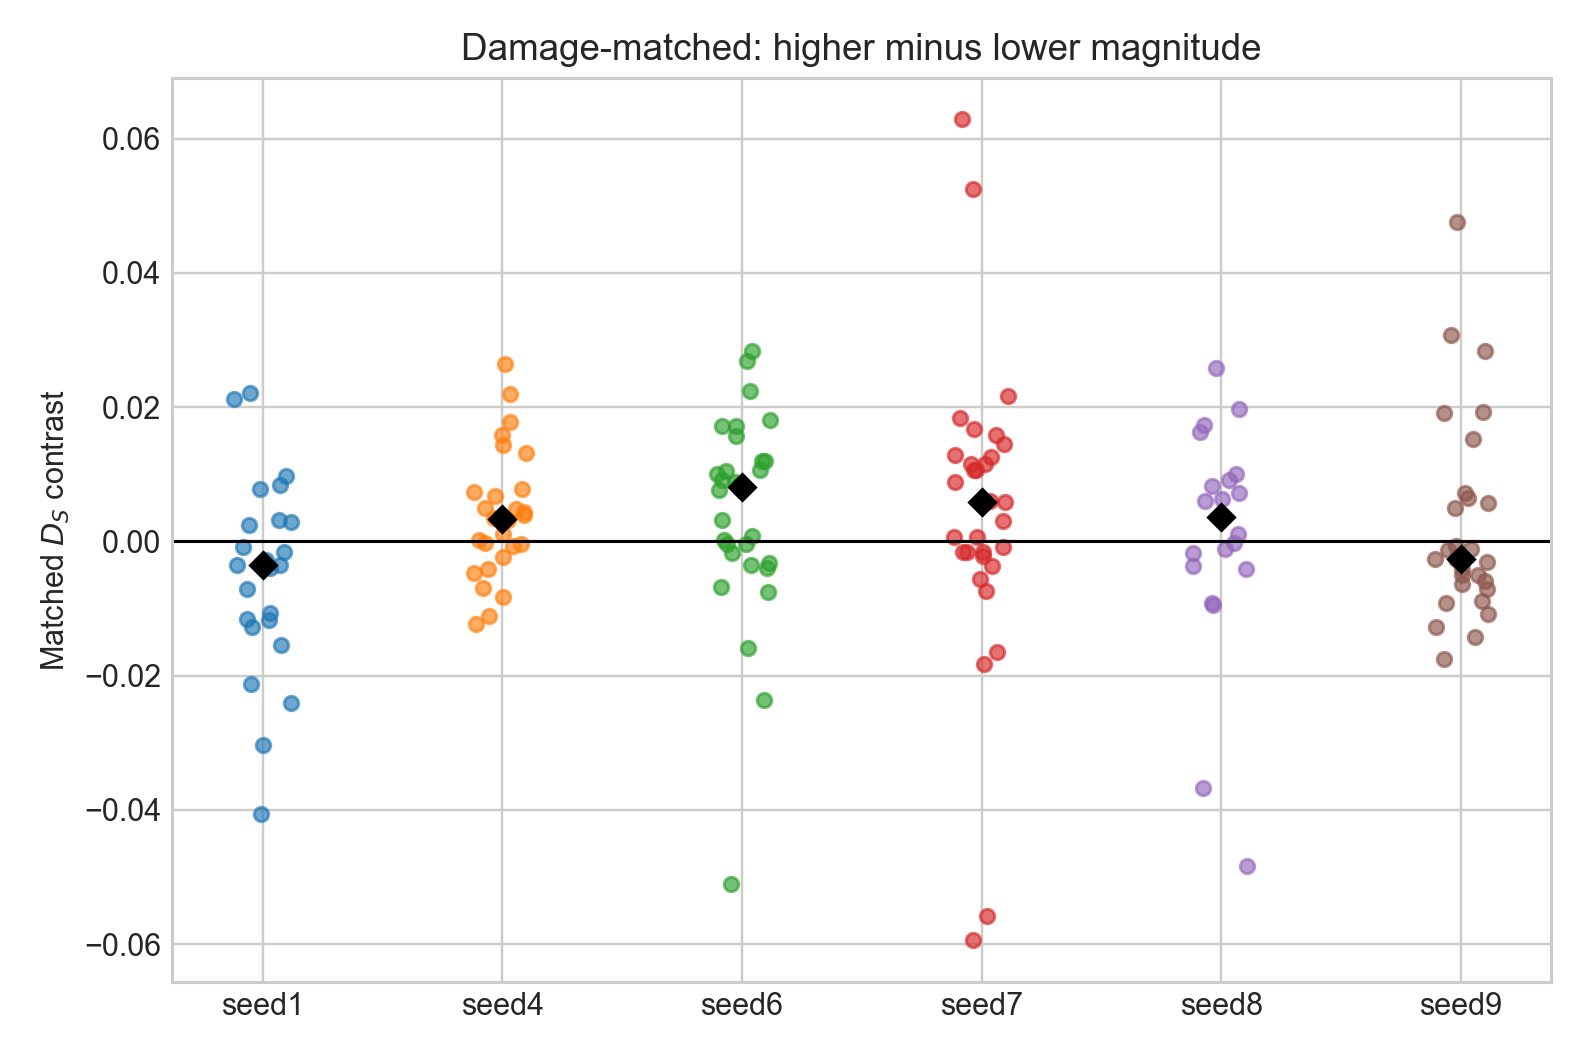
\includegraphics[width=\linewidth]{figures/draft2/fig2_damage_matched.png}
\\[-2mm]\small (b) Similar KL/NLL damage, different raw displacement
\end{minipage}
\caption{\textbf{Complementary matched contrasts within residual attenuation.}
Functional-damage differences retain a stable top-1 contrast at matched
magnitude, while the residual magnitude contrast is small after joint KL/NLL
matching. Points and intervals summarize independent runs, not tokens.}
\label{fig:damage}
\end{figure*}

Finally, KL, NLL, and $D_S$ are computed from the same intervened logits. The
matched design shows discrimination among measured descriptors; it does not
randomize KL/NLL or establish mediation.

\section{Functional Damage Does Not Eliminate Intervention-Family Dependence}
\label{sec:family}

The within-family result motivates the paper's central test. If output-level
damage is an adequate description of an intervention, then two structurally
different interventions matched on KL and NLL should have equivalent top-1
damage. We compare block attenuation with norm-controlled additive activation
noise after the intact block.

\paragraph{Qualitative replication in a second family.}
The noise family reproduces the early-to-late direction: all five independent
runs have negative $\deltas$, with mean $-0.07246$ and 95\% interval
$[-0.08438,-0.06304]$; all 25 eligible confidence-bin comparisons are negative.
This rules out the narrow claim that the sign is unique to literal block
bypass. It does not imply that the two families have the same quantitative
response. An initial post-hoc cross-family comparison in ARC-005 had only
26/150 strict matches and failed its match-quality gate; its residual is not
used as confirmatory evidence.

\paragraph{Prospective joint-damage targeting.}
For each block target at the same run, checkpoint, and layer, a blinded
one-dimensional search chooses the noise strength using only KL, NLL, strength,
and technical diagnostics. It never computes or records $D_S$. Strict Class A
support rises to 103/150 cells (68.7\%); the A+B sensitivity set contains
134/150 (89.3\%). Mean relative KL and NLL errors among Class A targets are
1.94\% and 1.87\%, respectively. Matching assignments and calipers are frozen
before top-1 outcomes are revealed.

\paragraph{Assay invalidation and repair.}
The first reveal was invalid. Historical block outcomes had used
`topk(2)[...,0]', whereas new noise outcomes used `argmax'. Exact FP16 ties can
resolve to different token indices; the maximum single-cell correction was
comparable with the invalid aggregate. Analysis stopped before downstream
geometry modeling. The original estimate is withdrawn.

ARC-006R changes only the identity convention: both families select the lowest
vocabulary index among exact maximum logits. It does not change targets,
matching classes, seeds, checkpoints, layers, equivalence bounds, exclusions,
or the statistical protocol. The repair shifts the invalid point estimate by
$+0.00240$ (12.49\% of its magnitude), demonstrating that the bug was
scientifically material.

\paragraph{Corrected residual.}
Under the canonical rule,
\begin{align}
 R_{\rm family}&=-0.016833,\\
 95\%\ \mathrm{CI}&=[-0.020045,-0.012616].
\end{align}
All five run medians are negative and every leave-one-run-out estimate remains
below the negative equivalence boundary. Because the residual is
$D_S^{\rm noise}-D_S^{\rm block}$, its negative sign means that block
attenuation changes more top-1 predictions than matched activation noise on
average, despite similar KL/NLL damage. The interval lies wholly outside the
frozen $\pm0.010742$ equivalence band. The A+B sensitivity estimate is
$-0.01816$ and is directionally consistent.

The aggregate is not cellwise universal: 24/103 corrected cells reverse sign,
and layer means range from negative to positive. The result is therefore a
run-level family component with substantial heterogeneity, not a deterministic
law for every layer and checkpoint.

\begin{figure*}[t]
\centering
\begin{minipage}[t]{0.46\textwidth}\centering
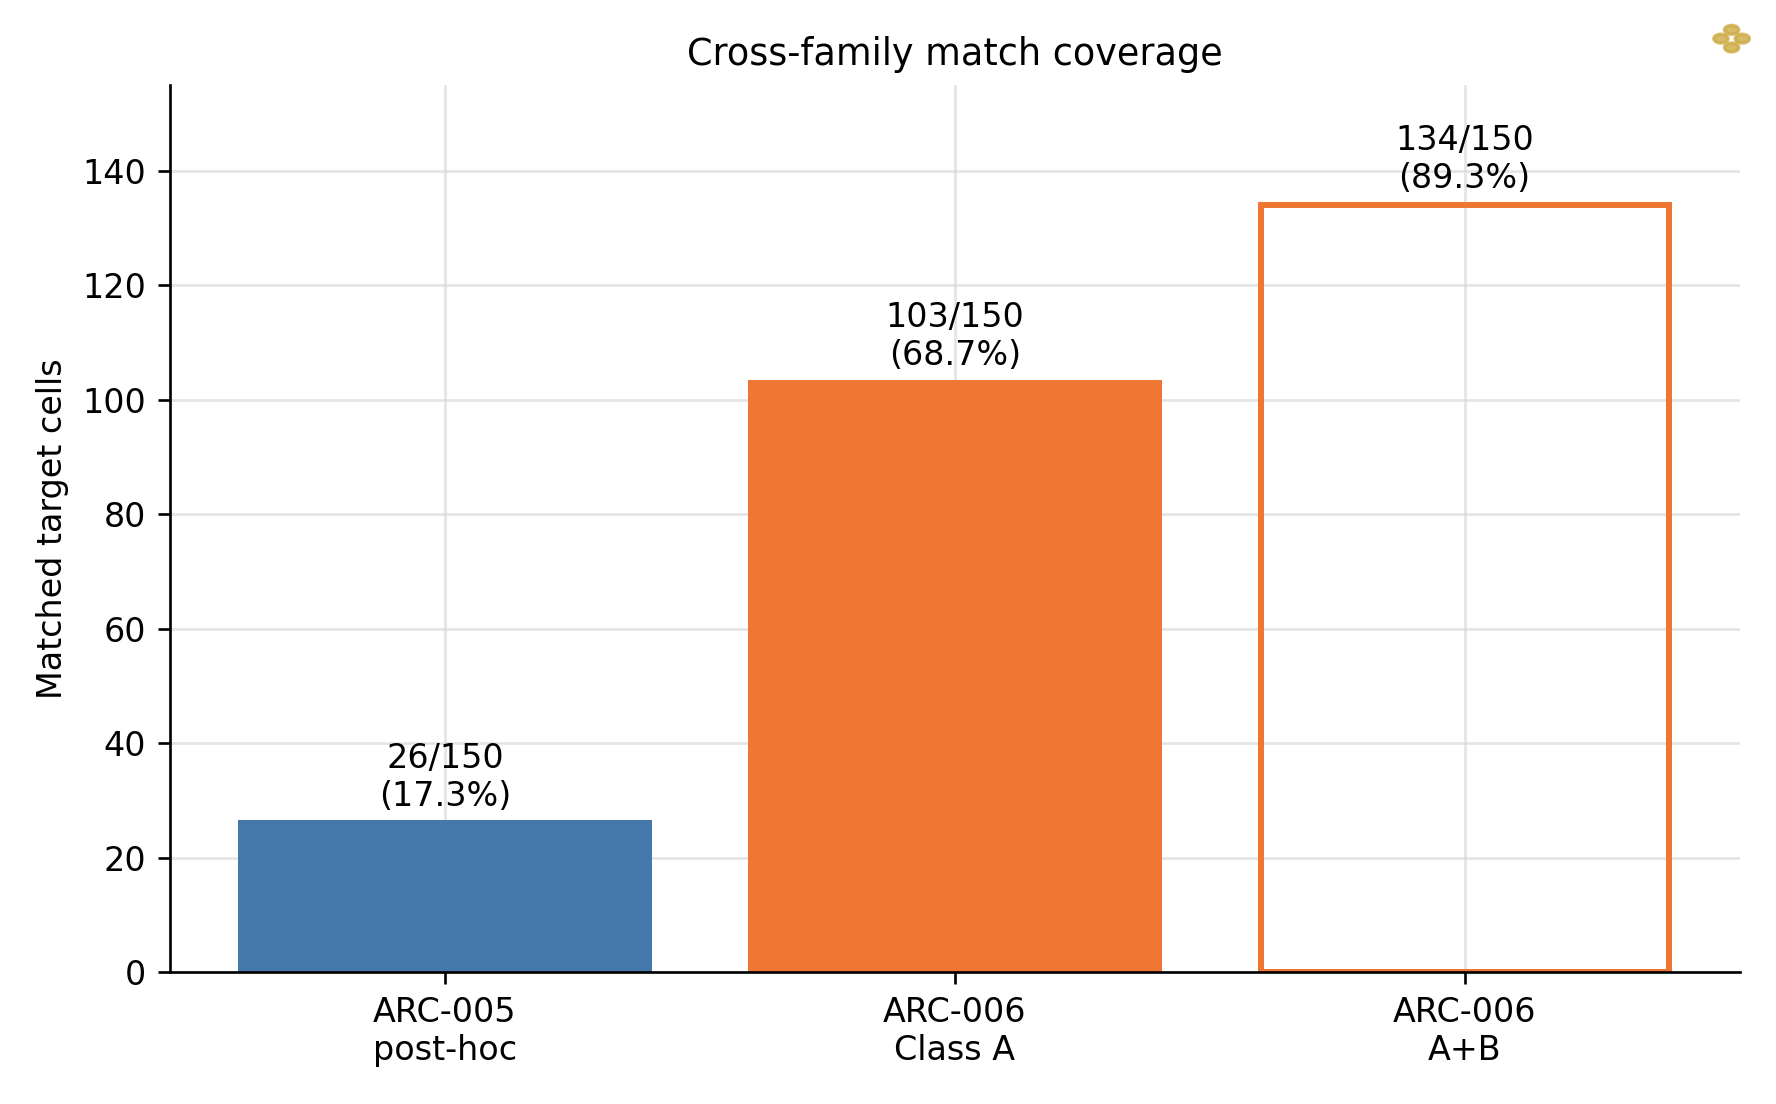
\includegraphics[width=\linewidth]{figures/draft2/fig3_match_coverage.png}
\\[-2mm]\small (a) Prospective matching support (outcome-independent)
\end{minipage}\hfill
\begin{minipage}[t]{0.50\textwidth}\centering
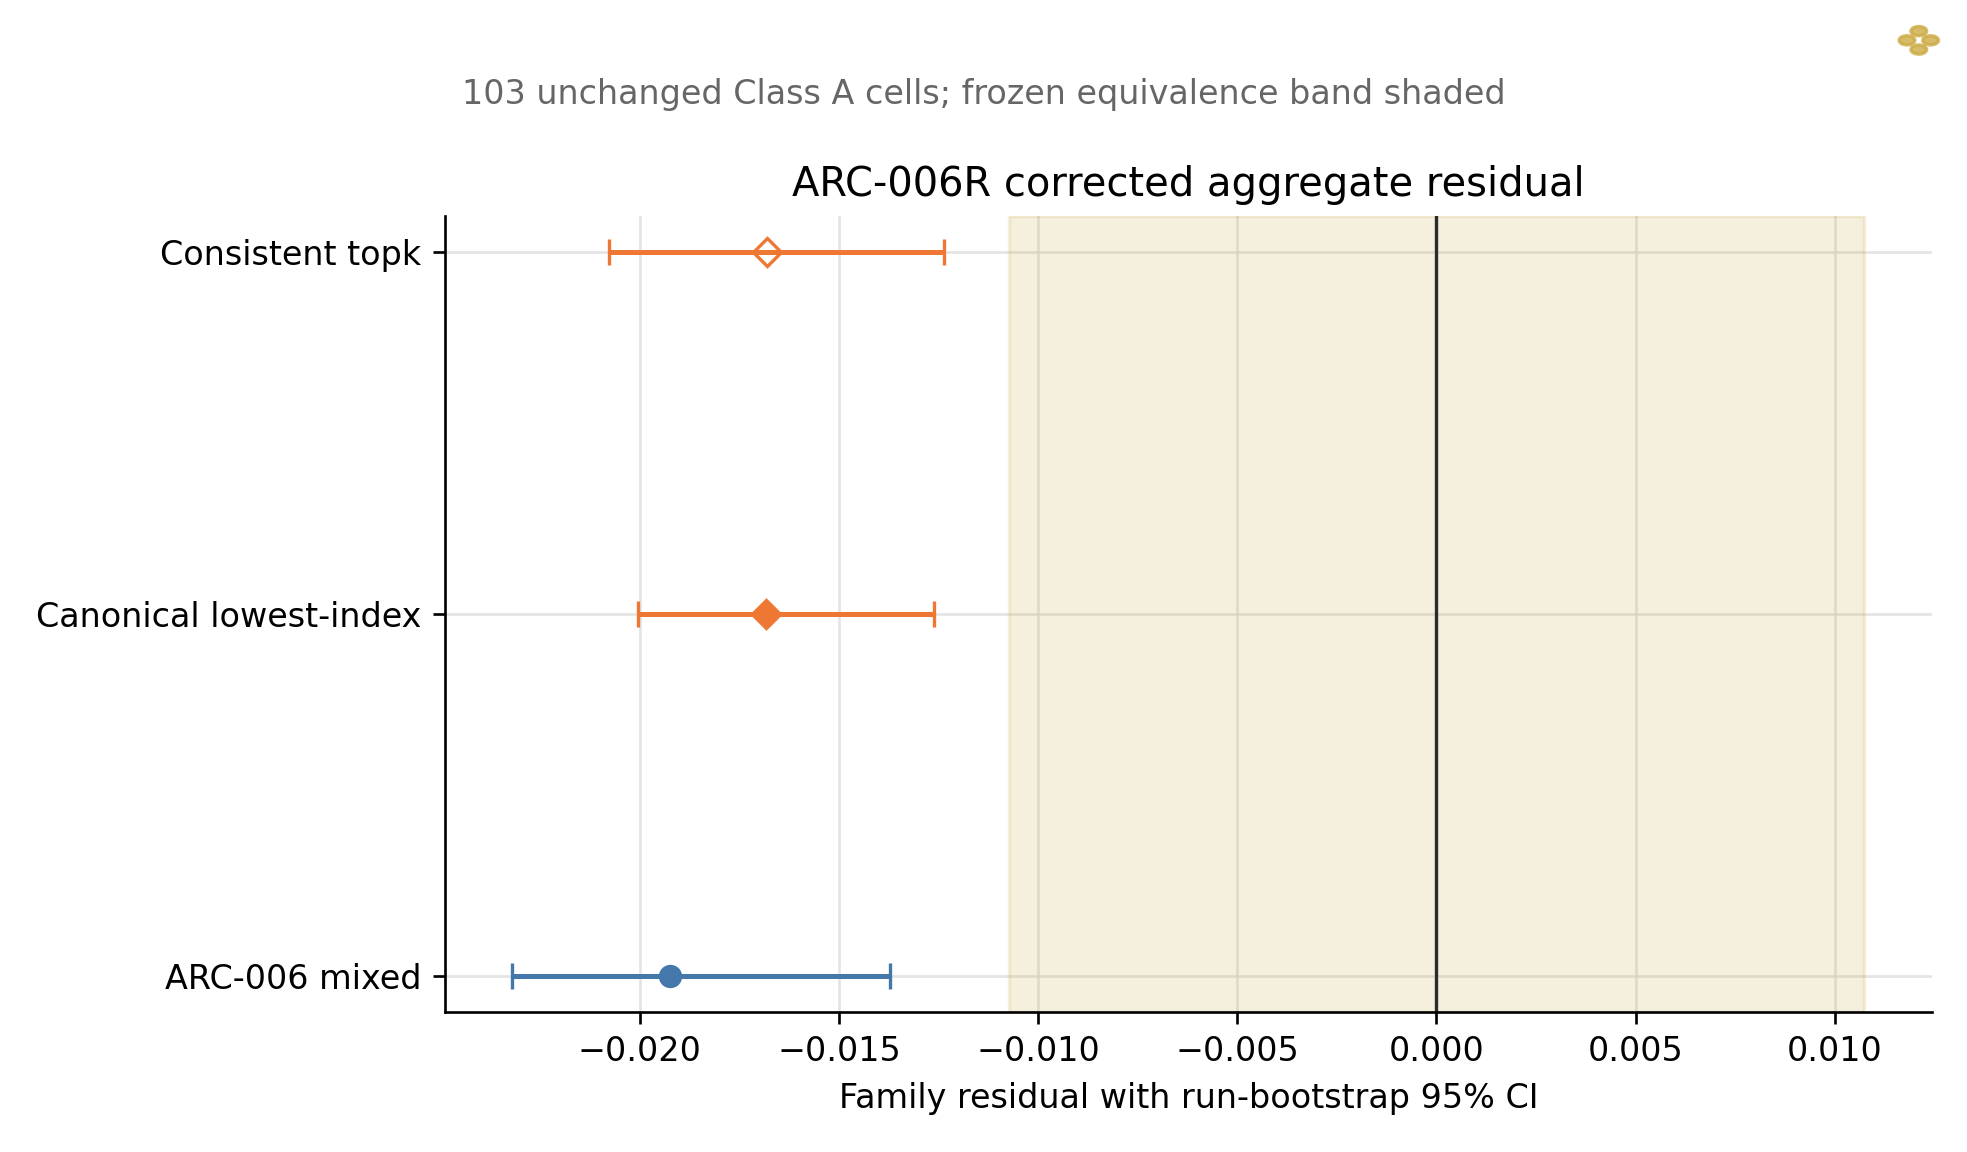
\includegraphics[width=\linewidth]{figures/draft2/fig3_corrected_residual.png}
\\[-2mm]\small (b) Corrected family residual under the canonical top-1 rule
\end{minipage}
\caption{\textbf{Predictive-damage matching does not eliminate family
dependence.} Panel (a) is a matching diagnostic and remains valid because the
assay repair did not change assignments. Panel (b) uses only corrected ARC-006R
outcomes; the withdrawn mixed-rule estimate is not shown as evidence.}
\label{fig:family}
\end{figure*}

The safe conclusion is limited but consequential: in this assay, KL and NLL
alignment is not sufficient to make the two interventions behaviorally
exchangeable. The result does not identify which unmeasured property carries
the difference.

\section{Simple Output Geometry Is Not Sufficient}
\label{sec:geometry}

The family residual may still be a simple artifact of the top-1 decision rule.
KL and NLL summarize the full predictive distribution, whereas $D_S$ depends
on whether a perturbation crosses the local argmax boundary. We therefore test
a frozen sequence of non-tautological output-geometry models on the corrected
103-cell support set.

The baseline model conditions on the functional-damage summary and fixed
run/checkpoint/layer effects. Adding the intact top-1 margin alone does not
change the family coefficient. Adding anchored boundary displacement also
fails to shrink it: the estimated magnitude grows by 1.49\%. A full block that
adds logit-change norm and absolute alignment reduces the family coefficient by
20.18\%, from approximately $-0.0168$ to $-0.01344$ (95\% interval
$[-0.01764,-0.00923]$). The point estimate remains outside the frozen
equivalence region, although its interval overlaps the boundary slightly.

The partial shrinkage is accompanied by counterevidence to a simple boundary
story. An outcome-blind geometry-matched subset covers 31/103 cells and retains
a residual of $-0.02436$ (95\% interval $[-0.03006,-0.01819]$). The geometry
features do not pass the frozen sign-reversal prediction gate (leave-one-run-out
AUC 0.664), and layer heterogeneity increases by 26.2\% after adjustment rather
than decreasing. The far-margin stratum is near zero, but the effect is largest
at medium rather than nearest margins.

\begin{figure*}[t]
\centering
\begin{minipage}[t]{0.48\textwidth}\centering
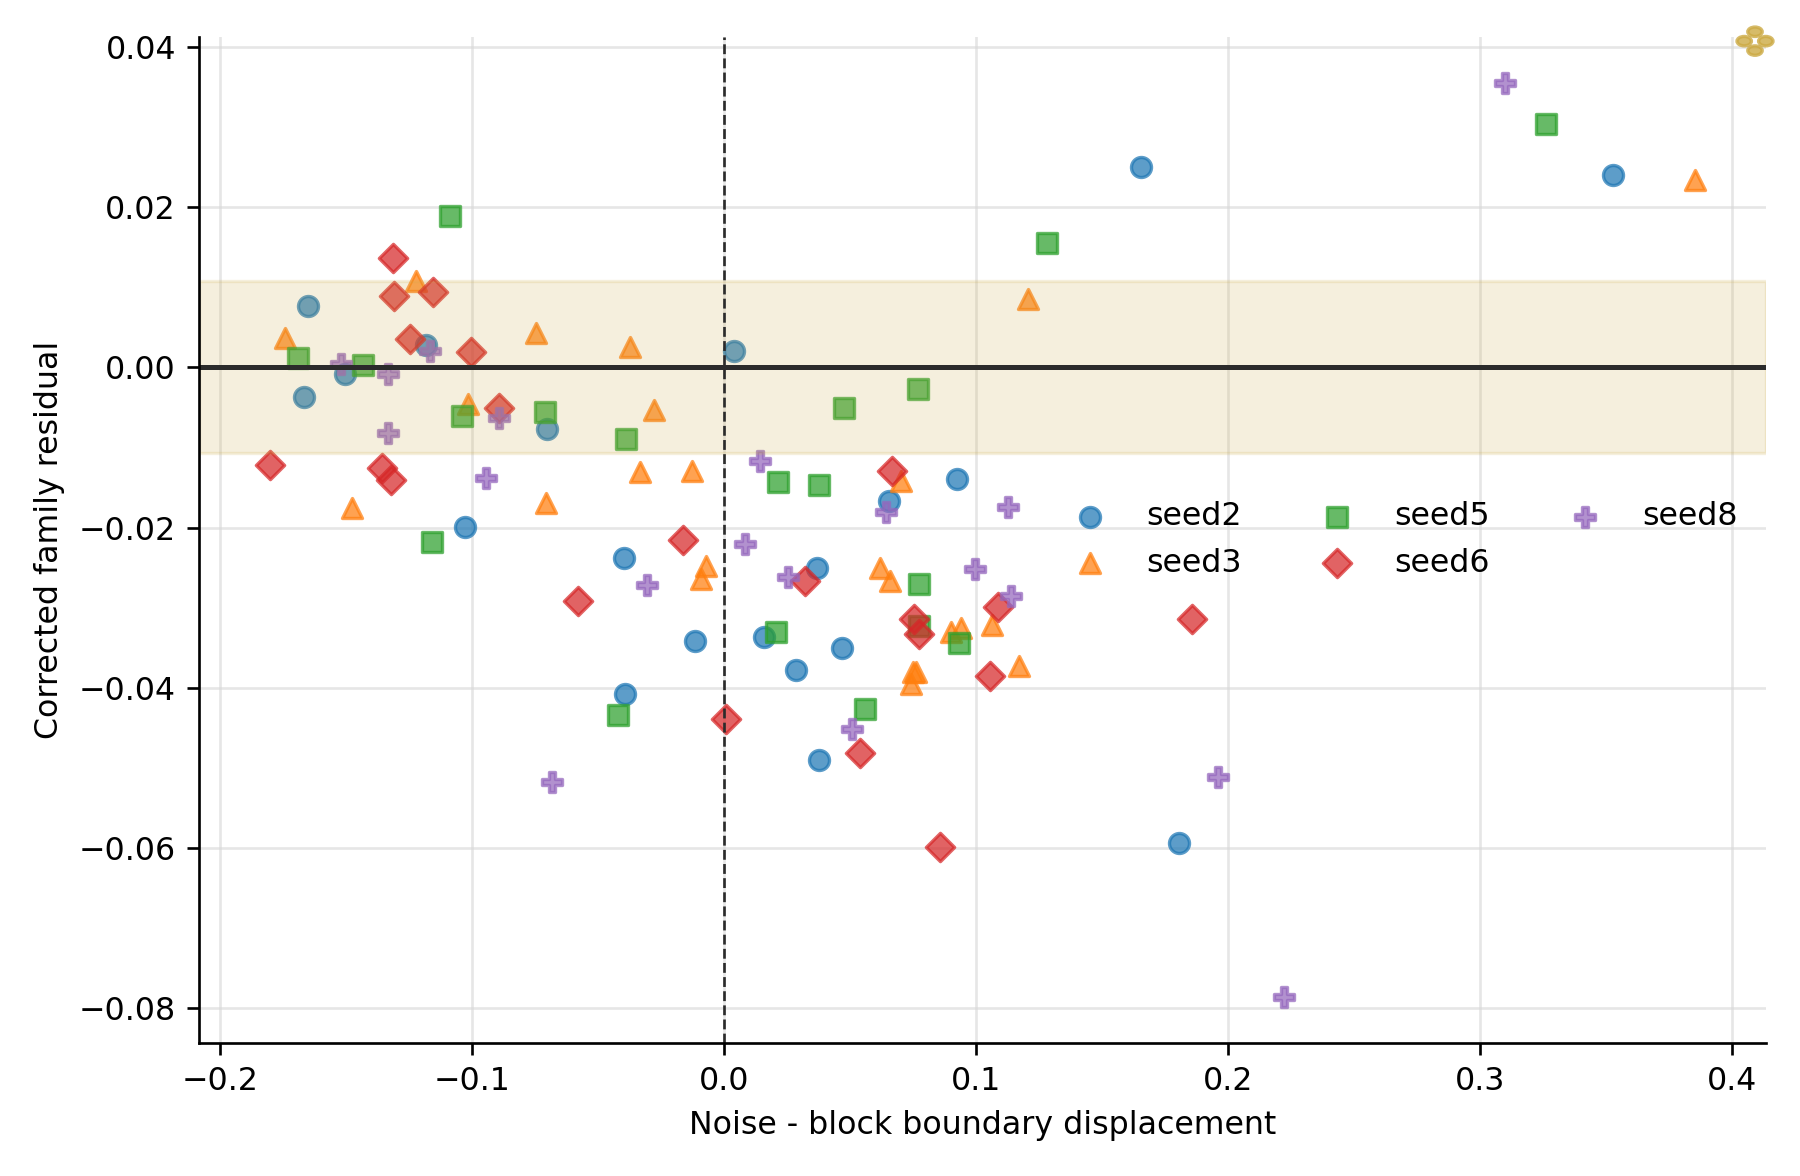
\includegraphics[width=\linewidth]{figures/draft2/fig4_residual_boundary.png}
\\[-2mm]\small (a) Frozen model sequence and residual shrinkage
\end{minipage}\hfill
\begin{minipage}[t]{0.48\textwidth}\centering
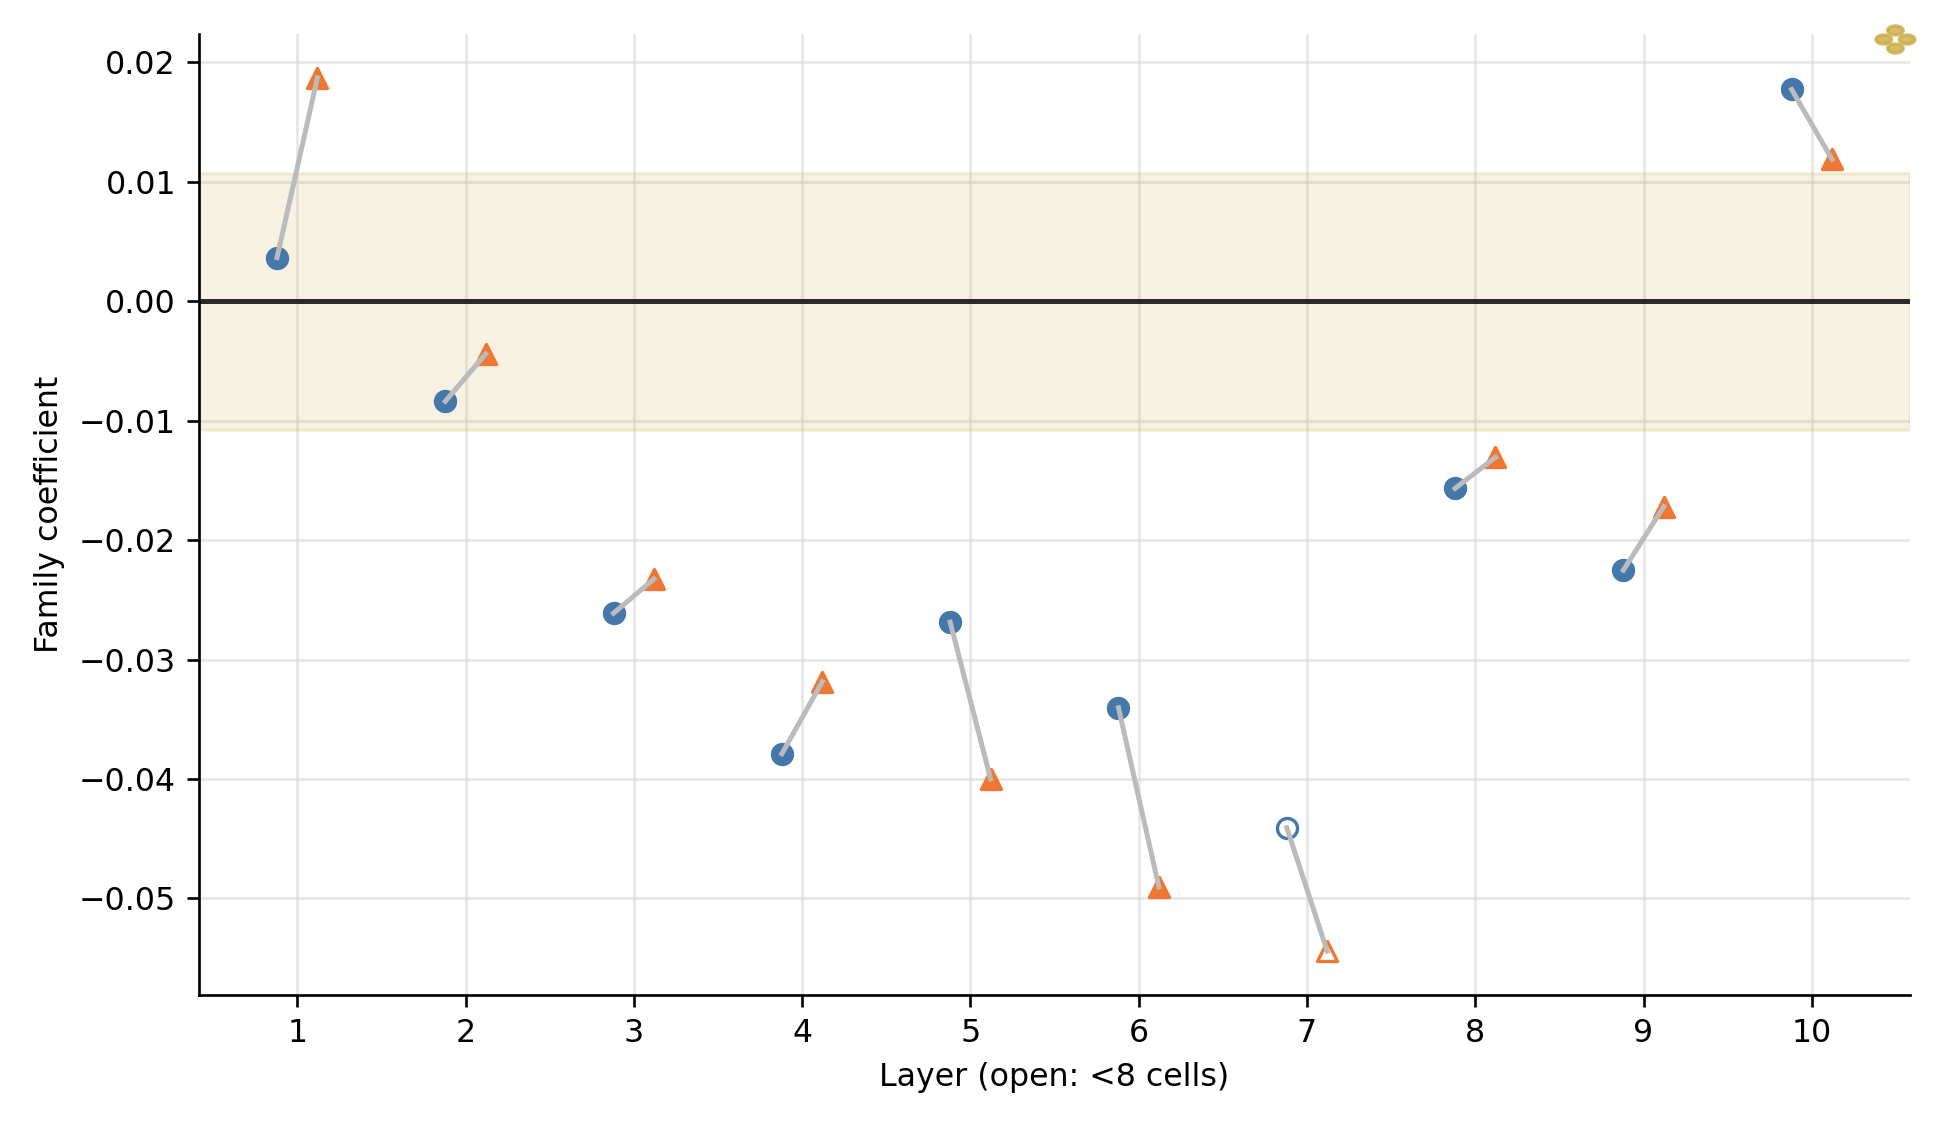
\includegraphics[width=\linewidth]{figures/draft2/fig4_layer_adjustment.png}
\\[-2mm]\small (b) Layer-level residual before and after geometry adjustment
\end{minipage}
\caption{\textbf{Output geometry is associated with only part of the family
residual.} The full frozen geometry block reduces the aggregate coefficient,
but the adjusted residual and heterogeneous layer structure remain. These are
associational controls, not a causal decomposition.}
\label{fig:geometry}
\end{figure*}

We conclude that the tested output geometry is incomplete. We do not conclude
that a deeper internal direction causes the remainder.

\section{Discussion and Limitations}

\subsection{Interventions as conditional measurements}

Raw displacement is insufficient within residual attenuation, and functional
damage is more informative, yet joint KL/NLL matching leaves a stable
block/noise difference. Intervention identity therefore retains information
not captured by either severity description; it is not itself an explanation.
A layer may look substitutable under one procedure and not another because the
procedures trace different paths through activation space. Intervention claims
should consequently report the model, data, family, magnitude convention,
functional-damage budget, response metric, and support diagnostics rather than
describe protocol-independent ``layer redundancy.''

\subsection{What remains unidentified}

The two families induce strongly different hidden perturbation directions, but
frozen observational direction features do not pass their preregistered
explanatory gates. A planned counterfactual direction test fails its support
gate before top-1 outcome reveal. We therefore make no causal claim about
internal direction; the blinded feasibility results remain in
Appendix~\ref{app:direction}.

\subsection{Limitations}

\paragraph{Scope.}
Evidence is limited to 70M/160M \model{} replicas, two English evaluation
streams with one tokenizer, and two intervention families; cross-family damage
matching is 160M and WikiText-2 only. Corpus magnitudes differ by about 23\%,
and replacement, interchange, attention-only, MLP-only, editing, other
architectures, and billion-parameter models remain untested.

\paragraph{Construct validity and heterogeneity.}
$S$ is discontinuous teacher-forced top-1 agreement, not semantic equivalence,
downstream capability, or pruning safety. KL, NLL, geometry, and $D_S$ share
logits, so matched associations may retain common metric geometry. Although the
aggregate family residual is seed-stable, 24/103 cells reverse sign and layer
effects vary; low support at layer 7 limits location-specific interpretation.

\paragraph{Mechanism and assay repair.}
The frozen tests weaken raw-magnitude, family-invariant damage, and simple
output-geometry accounts but do not identify an internal mechanism. The first
prospective reveal was invalidated by inconsistent FP16 top-1 tie handling; we
stopped, withdrew it, froze a family-independent lowest-index rule, and
recomputed without changing matches or exclusions. The corrected conclusion
survives, but the 12.49\% point-estimate change is material; full provenance is
in Appendix~\ref{app:repair}.

\section{Conclusion}

We tested whether protocol-dependent layer-intervention responses reduce to
raw magnitude or output-level predictive damage. Across independent small
\model{} runs and two streams, functional KL/NLL damage is more informative
than raw displacement within attenuation, yet prospective damage matching
leaves a corrected block/noise residual that simple output geometry only partly
explains. The mechanism remains unidentified; under the tested conditions,
intervention responses are protocol-conditioned measurements rather than
protocol-independent layer properties.

\subsection*{AI use statement}

Generative AI systems assisted with research-workflow orchestration,
literature triage, code generation and review, experiment-execution support,
analysis checks, and manuscript drafting and formatting. All cited literature,
reported numerical results, and manuscript claims were checked against
preserved sources and experiment artifacts; invalidated and inconclusive
analyses were not used to support the paper's claims. Generative AI was not
used to fabricate data, citations, or unexecuted results. The authors reviewed
all AI-assisted work and take responsibility for the final content, including
text, claims, code, and artifacts produced with generative-AI assistance.

\subsection*{Ethics statement}

This study analyzes publicly released language models and evaluation corpora.
It does not involve human participants, deployment, or external communication.
The principal research-integrity risk is overinterpreting intervention assays;
we address it by preserving invalidated analyses, separating associative from
causal evidence, and limiting claims to the tested models, corpora, and
interventions.

\subsection*{Reproducibility statement}

Section~\ref{sec:setup} defines the frozen assay and statistical units. The
appendix provides run-level summaries, matching diagnostics, confidence
controls, cross-corpus details, the assay invalidation and deterministic
top-1 repair, layer analyses, and artifact provenance. The accompanying
research artifacts retain preregistrations, commands, raw and processed
results, and figure-generating inputs for the validated analyses.


\bibliographystyle{iclr2027/iclr2027_conference}
\bibliography{references}

\appendix
\section{Full Run Tables}
\label{app:contract}

The machine-readable source of every number appearing in the main text is
`paper/numerical\_provenance.csv'. Full run-level outputs remain in the sealed
ARC directories rather than being copied or rounded again. The principal 160M
run table is `meta\_arc05/ARC-20260826-5060-003/results/run\_level\_results.csv';
the cross-corpus table is
`research/arc\_20260828\_5060\_011/processed/core\_run\_results.csv'.

\paragraph{Frozen run and checkpoint allocation.}
The principal trajectory uses nine 160M runs at steps 14k, 36k, 72k, 107k,
and 143k; scale confirmation uses five 70M runs. Within-family mechanism
comparisons use six 160M runs (pilot labels 1, 4, and 9; confirmatory labels 6,
7, and 8) at steps 14k, 72k, and 143k. Cross-family targeting uses runs 2, 3,
5, 6, and 8 at those three checkpoints.

\paragraph{Frozen selection and matching details.}
Three selection seeds each produce six sequences with 256 predicted positions,
giving 4,608 positions per checkpoint. Magnitude-matched pairs require relative
magnitude ratio at most 1.10 and absolute KL separation at least 0.03.
Damage-matched pairs require KL gap at most
$\max(0.01,0.10\bar D_{\rm KL})$ and NLL gap at most
$\max(0.015,0.10\bar D_{\rm NLL})$, plus layer separation at least three or
magnitude ratio at least 1.25. Cross-family targeting uses a deterministic grid
and bounded one-dimensional refinement; top-1 outcomes remain hidden until the
target manifest and analysis are sealed.

\section{Seed-Level Robustness}

The primary WikiText-2 endpoint is negative in 9/9 160M runs. All leave-one-run-
out medians remain negative. The held-out ninth run is negative in all three
evaluation selections. At 70M, 5/5 independent runs are negative. On the
HellaSwag-derived stream, 6/6 runs and 18/18 fixed evaluation resamples are
negative. For the corrected family residual, all five run medians are negative
and all leave-one-run-out estimates remain below the negative equivalence
boundary.

\section{Matching Diagnostics}

Within-family matching is performed without pair reuse and within run and
checkpoint. Primary magnitude matching yields 185 pairs; damage matching yields
162 pairs. Cross-family targeting obtains 103/150 strict Class A cells and
134/150 A+B cells. The strict-set mean relative KL and NLL target errors are
1.94\% and 1.87\%. Sixteen targets remain Class C. The worst target has 16.45\%
relative KL and 23.42\% relative NLL error and is excluded by the frozen class
rule, not by its outcome.

\section{Confidence Control}

Fixed intact-confidence bins are
$[0,.05),[.05,.1),[.1,.2),[.2,.4),[.4,1.01)$. The
WikiText-2 core has 45/45 negative eligible run--bin endpoint changes. The
activation-noise confirmation has 25/25 negative run--bin changes. The
HellaSwag-derived stream has 30/30 negative changes. Fixed bins reduce a known
composition difference but do not exactly match token difficulty.

\section{Cross-Corpus Details}

Both streams use 4,608 predicted positions per checkpoint and the same
tokenizer and sequence-selection procedure. WikiText-2 contains encyclopedia
prose; the HellaSwag-derived stream contains correct everyday-event
continuations. Mean intact NLL is lower and intact confidence higher on the
latter. Its mean absolute endpoint effect is 0.766 of the WikiText-2 reference,
with a bootstrap interval $[0.645,0.880]$. The functional-damage versus
raw-magnitude ordering repeats, but the damage-matched raw-magnitude contrast
is small and above zero on HellaSwag. We therefore say “replicates across the
tested corpora,” not “corpus invariant.”

\section{Assay Invalidation and Deterministic Top-1 Repair}
\label{app:repair}

ARC-006 compared historical block outcomes extracted with `topk' against new
noise outcomes extracted with `argmax'. Exact FP16 ties can choose different
indices. ARC-007 detected the discrepancy at its reproduction gate before any
geometry model was fit. The original $-0.019235$ residual and its reversal
counts are invalid.

ARC-006R freezes a family-independent rule: select the lowest token index among
exact maximum logits. It reuses the same 150 targets, classes, seeds,
checkpoints, layers, calipers, and equivalence band. The corrected primary
residual is $-0.016833$; a globally consistent `topk' sensitivity is
$-0.016797$. Their difference is below the frozen numerical-instability
threshold. The repair, source hashes, and output manifest are retained in the
ARC-006R directory.

\section{Layer Heterogeneity}

The core endpoint sign is negative for every run--layer pair, but magnitude is
location dependent. In the corrected cross-family set, weighted layer-mean
standard deviation is 0.01746 and the layer range crosses zero. Layer 7 has
only three strict matches and is marked low support. Output-geometry adjustment
does not reduce this heterogeneity.

\section{Sign-Reversal Analysis}

Twenty-four of 103 strict matched cells have
$D_S^{\rm noise}-D_S^{\rm block}>0$, despite the negative aggregate. A frozen
geometry classifier reaches leave-one-run-out AUC 0.664 and does not pass the
informativeness gate. These reversals are retained and prevent a uniform
cellwise family claim.

\section{Output-Geometry Details}

The preregistered model sequence adds intact margin, anchored boundary
displacement, then logit-change norm and absolute alignment. KL and NLL are
nearly collinear on the matched set, so the main regression uses a frozen
functional-damage summary rather than interpreting their separate
coefficients. The full geometry block shrinks the family coefficient by
20.18\%; the geometry-matched subset and reversal analysis provide negative
evidence against a complete output-boundary account.

\section{Internal-Direction Non-Identifiability}
\label{app:direction}

The hidden perturbation vectors for the two families are almost orthogonal.
Adding observational direction features to the frozen output-geometry baseline
improves held-out residual RMSE by 9.63\%, below the preregistered 10\% gate,
and changes reversal AUC by only 0.0026. The first counterfactual calibration
produces 15/103 jointly supported cells and fails before outcome reveal. The
paper therefore makes no statement about the sign or magnitude of a directional
causal effect.

\section{Continuous-Alpha Feasibility Failure}

ARC-009 uses continuous alpha to improve joint support without exposing
$D_S$. Strict PASS-A support rises from 15 to 47 cells and PASS-B reaches 29,
but the frozen minimum is not met and layer 2 has 0/15 PASS-A cells. The causal
branch terminates without a reveal; thresholds are not relaxed post hoc.

\section{Reproducibility and Provenance}

Every ARC stores preregistration or protocol documents, raw/processed results,
run manifests, commands, integrity hashes, and resource accounting. The Draft 0
provenance table records the exact artifact used for each number. GPU inference
is not rerun for manuscript construction. The empirical chain follows the
supersession rule ARC-006 $\rightarrow$ ARC-006R; later analyses reproduce the
corrected baseline before proceeding.


\end{document}
